\documentclass[11pt,a4paper]{article}

\usepackage[T1]{fontenc}
\usepackage[utf8]{inputenc}
\usepackage[english]{babel}
\usepackage[a4paper,top=2.15cm,bottom=2.25cm,left=2.4cm,right=2.4cm,headsep=12pt]{geometry}
\usepackage{amsmath,amssymb,mathtools}
\usepackage{enumitem}
\usepackage{eurosym}
\usepackage{graphicx}
\usepackage{xcolor}
\usepackage{microtype}
\usepackage{avant}
\usepackage{mathptmx}
\usepackage{titlesec}
\usepackage{fancyhdr}
\usepackage{mdframed}
\usepackage{tikz}
\usepackage{needspace}
\usepackage{hyperref}
\usetikzlibrary{arrows.meta,positioning}

\definecolor{PPEBurgundy}{RGB}{112,28,47}
\definecolor{PPENavarraRed}{RGB}{211,32,46}
\definecolor{PPEGold}{RGB}{185,143,57}
\definecolor{PPEAccentLight}{RGB}{248,235,238}
\definecolor{PPEInk}{RGB}{37,31,33}
\definecolor{PPEMuted}{RGB}{101,83,88}

\hypersetup{colorlinks=true,linkcolor=PPEBurgundy,urlcolor=PPEBurgundy}
\setlength{\parindent}{0pt}
\setlength{\parskip}{0.38em}
\setlist[itemize]{topsep=0.25em,itemsep=0.15em,leftmargin=1.45em}
\setlist[enumerate]{topsep=0.28em,itemsep=0.3em,leftmargin=1.8em}
\raggedbottom
\allowdisplaybreaks[2]

\titleformat{\section}
  {\sffamily\bfseries\large\color{PPEInk}}
  {\color{PPEBurgundy}\thesection}{0.8em}{}
\titlespacing*{\section}{0pt}{1.15em}{0.45em}

\newmdenv[
  skipabove=0.55em,skipbelow=0.7em,
  leftline=true,rightline=false,topline=false,bottomline=false,
  linewidth=3pt,linecolor=PPEBurgundy,backgroundcolor=PPEAccentLight,
  innerleftmargin=0.75em,innerrightmargin=0.75em,
  innertopmargin=0.5em,innerbottommargin=0.5em
]{instructionsbox}

\pagestyle{fancy}
\fancyhf{}
\fancyhead[LE,LO]{\sffamily\small Microeconomics \textbar{} Final Examination}
\fancyhead[RE,RO]{\sffamily\small\color{PPEBurgundy}\thepage}
\fancyfoot[C]{\sffamily\scriptsize\color{PPEMuted}Politics, Philosophy and Economics \textbar{} University of Navarra}
\renewcommand{\headrulewidth}{0.45pt}
\renewcommand{\headrule}{\hbox to\headwidth{\color{PPEGold}\leaders\hrule height \headrulewidth\hfill}}
\setlength{\headheight}{15pt}

\newcommand{\answerline}{\rule{0.34\textwidth}{0.35pt}}
\newcommand{\shortblank}{\rule{0.15\textwidth}{0.35pt}}
\newcommand{\mcq}[5]{%
  \item #1\hfill{\sffamily\scriptsize\color{PPEMuted}(1 point)}%
  \begin{enumerate}[label=\textbf{\Alph*.},leftmargin=1.7em,topsep=0.18em,itemsep=0.1em]
    \item #2
    \item #3
    \item #4
    \item #5
  \end{enumerate}%
}

\begin{document}

\begin{center}
  \IfFileExists{assets/branding/unav-logo-black.png}{%
    
\includegraphics[width=0.30\textwidth]{assets/branding/unav-logo-black.png}%
  }{%
    {\sffamily\bfseries\Large Universidad de Navarra}%
  }\par
  \vspace{0.35em}
  {\color{PPEGold}\rule{0.74\textwidth}{1.3pt}\par}
  \vspace{0.45em}
  {\sffamily\bfseries\color{PPEBurgundy}\LARGE Final Examination: Microeconomics\par}
  \vspace{0.12em}
  {\sffamily\large Full course \textbar{} 100 points\par}
\end{center}

\begin{instructionsbox}
\textbf{Instructions.} Answer every question and show your work in the
problems. All mathematical calculations have been designed to be completed
without a calculator. For the 33 multiple-choice questions, a correct answer
earns \(+1\) point, a wrong answer earns \(-0.25\) points, and a blank answer
earns \(0\) points. For diagrams, label axes and relevant curves or points.
\end{instructionsbox}

\textbf{Name and surname:} \rule{0.62\textwidth}{0.35pt}

\section{Multiple-choice questions \hfill (33 points)}

Mark one answer in each row.

\begin{center}
\renewcommand{\arraystretch}{1.35}
\small
\begin{tabular}{c|cccc@{\qquad}c|cccc@{\qquad}c|cccc}
 & A & B & C & D & & A & B & C & D & & A & B & C & D\\ \hline
1 & \(\circ\) & \(\circ\) & \(\circ\) & \(\circ\) &
12 & \(\circ\) & \(\circ\) & \(\circ\) & \(\circ\) &
23 & \(\circ\) & \(\circ\) & \(\circ\) & \(\circ\)\\
2 & \(\circ\) & \(\circ\) & \(\circ\) & \(\circ\) &
13 & \(\circ\) & \(\circ\) & \(\circ\) & \(\circ\) &
24 & \(\circ\) & \(\circ\) & \(\circ\) & \(\circ\)\\
3 & \(\circ\) & \(\circ\) & \(\circ\) & \(\circ\) &
14 & \(\circ\) & \(\circ\) & \(\circ\) & \(\circ\) &
25 & \(\circ\) & \(\circ\) & \(\circ\) & \(\circ\)\\
4 & \(\circ\) & \(\circ\) & \(\circ\) & \(\circ\) &
15 & \(\circ\) & \(\circ\) & \(\circ\) & \(\circ\) &
26 & \(\circ\) & \(\circ\) & \(\circ\) & \(\circ\)\\
5 & \(\circ\) & \(\circ\) & \(\circ\) & \(\circ\) &
16 & \(\circ\) & \(\circ\) & \(\circ\) & \(\circ\) &
27 & \(\circ\) & \(\circ\) & \(\circ\) & \(\circ\)\\
6 & \(\circ\) & \(\circ\) & \(\circ\) & \(\circ\) &
17 & \(\circ\) & \(\circ\) & \(\circ\) & \(\circ\) &
28 & \(\circ\) & \(\circ\) & \(\circ\) & \(\circ\)\\
7 & \(\circ\) & \(\circ\) & \(\circ\) & \(\circ\) &
18 & \(\circ\) & \(\circ\) & \(\circ\) & \(\circ\) &
29 & \(\circ\) & \(\circ\) & \(\circ\) & \(\circ\)\\
8 & \(\circ\) & \(\circ\) & \(\circ\) & \(\circ\) &
19 & \(\circ\) & \(\circ\) & \(\circ\) & \(\circ\) &
30 & \(\circ\) & \(\circ\) & \(\circ\) & \(\circ\)\\
9 & \(\circ\) & \(\circ\) & \(\circ\) & \(\circ\) &
20 & \(\circ\) & \(\circ\) & \(\circ\) & \(\circ\) &
31 & \(\circ\) & \(\circ\) & \(\circ\) & \(\circ\)\\
10 & \(\circ\) & \(\circ\) & \(\circ\) & \(\circ\) &
21 & \(\circ\) & \(\circ\) & \(\circ\) & \(\circ\) &
32 & \(\circ\) & \(\circ\) & \(\circ\) & \(\circ\)\\
11 & \(\circ\) & \(\circ\) & \(\circ\) & \(\circ\) &
22 & \(\circ\) & \(\circ\) & \(\circ\) & \(\circ\) &
33 & \(\circ\) & \(\circ\) & \(\circ\) & \(\circ\)
\end{tabular}
\end{center}

\begin{enumerate}[label=\textbf{\arabic*.},leftmargin=1.55em,itemsep=0.38em]
\small
  \mcq{Scarcity exists because}{all goods have a positive price.}{resources are limited relative to human wants.}{firms always make losses.}{governments set taxes.}
  \mcq{The opportunity cost of an action is}{the monetary payment actually made.}{the total benefit obtained.}{the value of the best alternative forgone.}{a cost that has already been paid.}
  \mcq{Transitivity requires that}{every bundle is strictly preferred to itself.}{if \(A\succeq B\) and \(B\succeq C\), then \(A\succeq C\).}{consumers prefer more of every good.}{all consumers rank bundles in the same way.}
  \mcq{The marginal rate of substitution measures}{the market price of a good.}{the amount of one good a consumer is willing to give up for another while holding utility constant.}{the marginal product of labour.}{the change in income after a price change.}
  \mcq{A change in a good's own price causes}{a shift of its demand curve.}{a movement along its demand curve.}{a shift of its supply curve.}{no change in quantity demanded.}
  \mcq{A normal good is one for which demand}{falls when income rises.}{rises when income rises, ceteris paribus.}{rises when its own price rises.}{is independent of income.}
  \mcq{A Giffen good is necessarily}{an inferior good whose demand can rise with its own price.}{a normal good with unit elasticity.}{a good with perfectly elastic demand.}{a good supplied by a monopoly.}
  \mcq{On a linear demand curve, total revenue is maximised where demand is}{perfectly inelastic.}{unit elastic.}{perfectly elastic.}{always negative.}
  \mcq{A production function has constant returns to scale if}{doubling all inputs doubles output.}{doubling labour doubles output while capital is fixed.}{marginal product is constant.}{average cost is constant.}
  \mcq{The MRTS of labour for capital is}{the ratio of input prices only.}{the rate at which labour can replace capital while holding output constant.}{the marginal cost of labour.}{the rate at which output changes with income.}
  \mcq{Fixed cost is}{a cost that varies with output.}{a cost that does not vary with output in the relevant period.}{always avoidable in the short run.}{equal to marginal cost.}

  \newpage
  \mcq{A competitive firm shuts down in the short run when}{price is below average variable cost.}{price is below average total cost.}{marginal cost is positive.}{fixed cost is positive.}
  \mcq{A perfectly competitive firm is a price taker because}{it produces no output.}{it is the only seller.}{it faces a market price it cannot individually influence.}{it chooses the price equal to marginal revenue.}
  \mcq{Consumer surplus is}{revenue minus total cost.}{the difference between willingness to pay and the price paid.}{the government's tax revenue.}{the firm's fixed cost.}
  \mcq{A single-price monopolist maximises profit where}{price equals average cost.}{marginal revenue equals marginal cost.}{demand is perfectly elastic.}{total revenue is zero.}
  \mcq{In a Cournot duopoly, firms choose}{prices simultaneously.}{quantities simultaneously.}{only their fixed costs.}{the same quantity by assumption.}
  \mcq{A general equilibrium describes}{a single market in which one firm sets price.}{a situation in which all interrelated markets clear simultaneously.}{a situation in which every consumer has the same income.}{a government policy that fixes every price.}
  \mcq{A negative externality exists when}{a private action imposes an uncompensated cost on others.}{a firm has fixed costs.}{demand is perfectly inelastic.}{all benefits are private.}
  \mcq{Adverse selection arises when}{hidden information exists before a contract or trade.}{hidden actions occur after a contract.}{all buyers have identical information.}{a bidder wins an auction.}
  \mcq{Moral hazard arises when}{a hidden action after a contract changes incentives.}{a buyer knows more before trade.}{all contracts are complete.}{prices are regulated.}
  \mcq{A dominant strategy is one that}{is best only when the rival cooperates.}{is best regardless of the opponents' actions.}{always yields the highest payoff in the entire matrix.}{must be played in every Nash equilibrium.}
  \mcq{A Nash equilibrium is an outcome where}{all players earn equal payoffs.}{no player can gain by changing strategy alone.}{players choose their dominant strategies.}{players maximise joint payoff.}
  \mcq{A subgame-perfect Nash equilibrium}{is a Nash equilibrium that prescribes optimal play in every subgame.}{requires every player to cooperate.}{exists only in simultaneous games.}{always gives equal payoffs.}
  \mcq{Mechanism design starts by asking}{how a planner can design rules that elicit desired behaviour.}{how firms set marginal cost.}{how consumers draw budget lines.}{how to avoid using incentives.}
  \mcq{In a first-price sealed-bid auction}{the winner pays the second-highest bid.}{the winner pays their own bid.}{all bidders pay their bids.}{the seller announces the price and lowers it over time.}
  \mcq{In a second-price sealed-bid auction}{the winner pays their own bid.}{the winner pays the lowest bid.}{the winner pays the second-highest bid.}{all bidders pay the average bid.}
  \mcq{In an English auction}{the price falls until a buyer accepts.}{bidders observe ascending bids in real time.}{all bids are sealed and simultaneous.}{the winner pays the lowest bid.}
  \mcq{System 1 thinking is typically}{fast, automatic, and intuitive.}{slow, deliberate, and effortful.}{fully rational and unbiased.}{used only for mathematical problems.}
  \mcq{The availability heuristic involves}{judging likelihood by how easily examples come to mind.}{preferring losses to gains.}{valuing a good more after owning it.}{always choosing the default option.}
  \mcq{Anchoring occurs when}{an initial value unduly influences later judgments.}{people ignore all reference points.}{a person treats all losses equally.}{future rewards are preferred to present rewards.}
  \mcq{Loss aversion means that}{losses are felt more strongly than equal-sized gains.}{people never take risks.}{gains and losses receive equal weight.}{people ignore sunk costs.}
  \mcq{Present bias is the tendency to}{prefer a smaller reward now to a larger reward later.}{save every current income increase.}{estimate probabilities from base rates only.}{choose only familiar brands.}
  \mcq{A framing effect occurs when}{equivalent information changes choices because it is presented differently.}{a person bids truthfully in an auction.}{a firm sets price equal to marginal cost.}{a consumer has convex preferences.}
\end{enumerate}

\newpage
\section{Utility maximisation \hfill (10 points)}

A consumer has income \(I=\text{\euro}160\) and chooses two goods,
\(x_1\) and \(x_2\). Their prices are \(p_1=\text{\euro}20\) and
\(p_2=\text{\euro}10\). Preferences are represented by
\[
u(x_1,x_2)=x_1^{1/4}x_2^{3/4}.
\]

\begin{enumerate}[label=\textbf{\alph*.}]
  \item Write and draw the budget line, labelling its intercepts and slope.
        \hfill (2 points)
  \item Substitute the budget constraint into the utility function and find
        the utility-maximising bundle. Show the derivative. \hfill (4 points)
  \item Solve the same problem using the tangency condition
        \(\mathrm{MRS}_{1,2}=p_1/p_2\). \hfill (4 points)
\end{enumerate}

\begin{center}
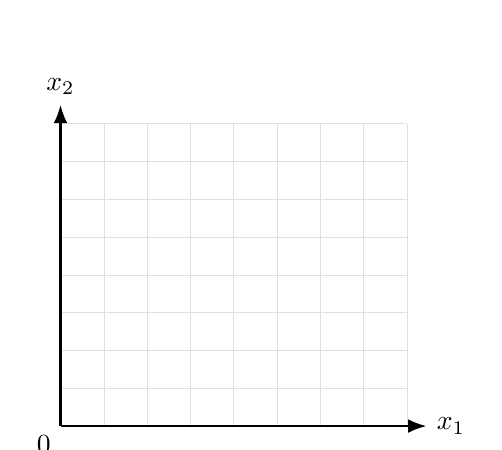
\begin{tikzpicture}[x=0.55cm,y=0.24cm,>=Latex]
  \foreach \x in {0,...,8}
    \draw[gray!24,very thin] (\x,0) -- (\x,16);
  \foreach \y in {0,2,...,16}
    \draw[gray!24,very thin] (0,\y) -- (8,\y);
  \draw[->,thick] (0,0) -- (8.45,0) node[right] {\(x_1\)};
  \draw[->,thick] (0,0) -- (0,17.0) node[above] {\(x_2\)};
  \node[below left] at (0,0) {\(0\)};
\end{tikzpicture}
\end{center}

\newpage
\section{Cost minimisation and cost curves \hfill (8 points)}

\textbf{35.a Cost-minimising inputs.} A firm has production function
\[
q=\sqrt{LK}.
\]
The wage is \(w=\text{\euro}4\), the rental price of capital is
\(r=\text{\euro}1\), and the firm must produce \(q=12\).

\begin{enumerate}[label=(\roman*)]
  \item Find the cost-minimising bundle \((L^*,K^*)\). \hfill (2 points)
  \item Calculate the minimum cost. \hfill (1 point)
\end{enumerate}

\textbf{35.b Cost curves and output choice.} A price-taking firm has
\[
TC(q)=36+6q+q^2
\]
and faces \(p=\text{\euro}30\).

\begin{enumerate}[label=(\roman*)]
  \item Find \(FC\), \(VC(q)\), \(MC(q)\), \(AFC(q)\), \(AVC(q)\), and
        \(ATC(q)\). \hfill (2 points)
  \item Find the profit-maximising output. \hfill (1 point)
  \item At that output, calculate \(ATC\) and profit. Should the firm operate
        in the short run? \hfill (2 points)
\end{enumerate}

\newpage
\section{Production technology and MRTS \hfill (7 points)}

A workshop has production function
\[
q=4L^{1/2}K^{1/2},
\]
where \(L\) is labour and \(K\) is capital.

\begin{enumerate}[label=\textbf{\alph*.}]
  \item Find \(MP_L\), \(MP_K\), and \(\mathrm{MRTS}_{L,K}=MP_L/MP_K\).
        \hfill (3 points)
  \item At \(L=4\) and \(K=9\), calculate \(q\), \(MP_L\), \(MP_K\), and
        \(\mathrm{MRTS}_{L,K}\). \hfill (3 points)
  \item Does the technology display increasing, constant, or decreasing
        returns to scale? Demonstrate your answer. \hfill (1 point)
\end{enumerate}

\newpage
\section{Elasticity, revenue, and the Laffer curve \hfill (10 points)}

\textbf{37.a Elasticity and a firm's revenue.} Demand for cinema tickets is
\[
Q=120-2P.
\]
At \(P=\text{\euro}20\), calculate the price elasticity of demand using
\(\varepsilon=(dQ/dP)(P/Q)\). Is demand elastic or inelastic? If price rises
slightly, what happens to total revenue? \hfill (3 points)

\vspace{0.6em}
\textbf{37.b Tax revenue.} A per-unit tax \(t\) raises the price paid by
buyers and reduces market demand according to
\[
Q(t)=40-2t,\qquad 0\leq t\leq20.
\]
Government revenue is \(R(t)=tQ(t)\).

\begin{enumerate}[label=(\roman*)]
  \item Write \(R(t)\) as a function of \(t\). \hfill (2 points)
  \item Find the tax \(t^*\) that maximises government revenue. \hfill (2 points)
  \item Calculate \(Q(t^*)\) and \(R(t^*)\). \hfill (1 point)
  \item Draw the Laffer curve, with \(t\) on the horizontal axis and
        \(R(t)\) on the vertical axis. Mark \(t^*\). \hfill (2 points)
\end{enumerate}

\begin{center}
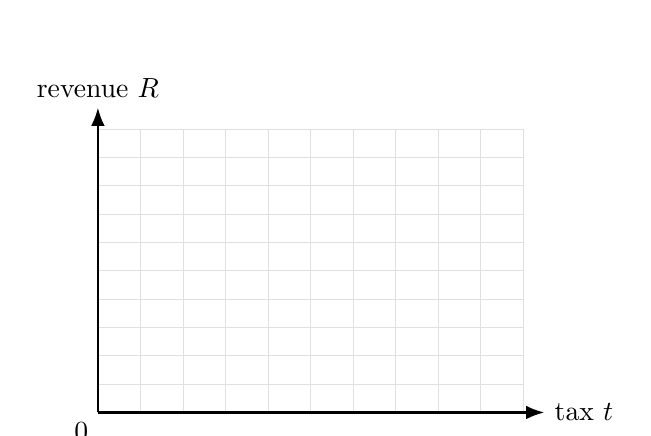
\begin{tikzpicture}[x=0.27cm,y=0.018cm,>=Latex]
  \foreach \x in {0,2,...,20}
    \draw[gray!24,very thin] (\x,0) -- (\x,200);
  \foreach \y in {0,20,...,200}
    \draw[gray!24,very thin] (0,\y) -- (20,\y);
  \draw[->,thick] (0,0) -- (21.0,0) node[right] {tax \(t\)};
  \draw[->,thick] (0,0) -- (0,215) node[above] {revenue \(R\)};
  \node[below left] at (0,0) {\(0\)};
\end{tikzpicture}
\end{center}

\newpage
\section{Game theory \hfill (15 points)}

In every matrix, payoffs are written as \((A,B)\), with the row player listed
first. Each game is worth 3 points.

\textbf{38.a Prisoner's Dilemma.} Identify each player's dominant strategy,
the Nash equilibrium, and the Pareto-superior outcome.

\begin{center}
\renewcommand{\arraystretch}{1.45}
\begin{tabular}{c|c|c}
 & B: Cooperate & B: Defect \\ \hline
A: Cooperate & \((3,3)\) & \((0,5)\)\\
A: Defect & \((5,0)\) & \((1,1)\)
\end{tabular}
\end{center}

\textbf{38.b Stag Hunt.} Find all pure-strategy Nash equilibria. Which
equilibrium is payoff dominant?

\begin{center}
\renewcommand{\arraystretch}{1.45}
\begin{tabular}{c|c|c}
 & B: Stag & B: Hare \\ \hline
A: Stag & \((4,4)\) & \((0,3)\)\\
A: Hare & \((3,0)\) & \((3,3)\)
\end{tabular}
\end{center}

\newpage
\textbf{38.c Dominated strategies in a \(3\times3\) game.} Identify any
strictly dominated strategies. Then find the pure-strategy Nash equilibrium.

\begin{center}
\renewcommand{\arraystretch}{1.45}
\begin{tabular}{c|c|c|c}
 & B: Left & B: Centre & B: Right \\ \hline
A: Up & \((4,2)\) & \((2,1)\) & \((1,0)\)\\
A: Centre & \((5,4)\) & \((3,3)\) & \((2,2)\)\\
A: Down & \((2,3)\) & \((1,2)\) & \((0,1)\)
\end{tabular}
\end{center}

\vspace{1.0em}
\textbf{38.d Non-symmetric \(3\times3\) game.} Find all pure-strategy Nash
equilibria.

\begin{center}
\renewcommand{\arraystretch}{1.45}
\begin{tabular}{c|c|c|c}
 & B: Left & B: Middle & B: Right \\ \hline
A: A & \((6,5)\) & \((1,0)\) & \((2,1)\)\\
A: B & \((0,1)\) & \((5,6)\) & \((1,2)\)\\
A: C & \((2,0)\) & \((0,2)\) & \((4,4)\)
\end{tabular}
\end{center}

\newpage
\textbf{38.e Extensive-form game.} Use backward induction to find the unique
subgame-perfect Nash equilibrium (SPNE).

\begin{center}
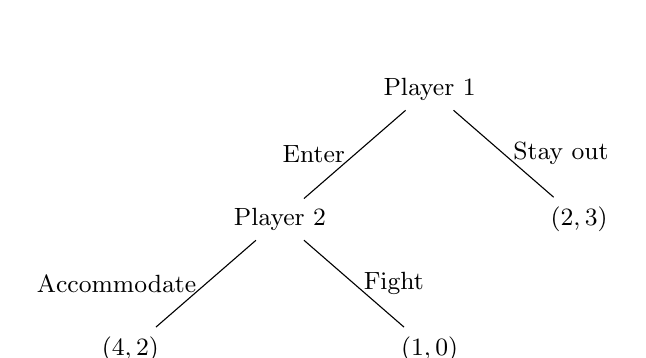
\begin{tikzpicture}[>=Latex,level distance=1.65cm,sibling distance=3.8cm,
  every node/.style={font=\small}]
  \node {Player 1}
    child {node {Player 2}
      child {node {\((4,2)\)}
        edge from parent node[left] {Accommodate}}
      child {node {\((1,0)\)}
        edge from parent node[right] {Fight}}
      edge from parent node[left] {Enter}}
    child {node {\((2,3)\)}
      edge from parent node[right] {Stay out}};
\end{tikzpicture}
\end{center}

\vfill
\newpage
\section{Fill in the text \hfill (4 points)}

Write one precise term or short phrase in each blank.

\begin{enumerate}[label=\textbf{\alph*.},itemsep=1.2em]
  \item In Kahneman's dual-process theory, System 1 is fast, automatic, and
        \answerline.
  \item Judging the probability of an event by how easily examples come to
        mind is the \answerline.
  \item In a second-price sealed-bid auction, the winner pays the
        \answerline.
  \item In a first-price sealed-bid auction, the winner pays
        \answerline.
\end{enumerate}

\section{Market failures: a positive externality \hfill (3 points)}

The private marginal benefit from a vaccination is
\[
PMB=40-Q,
\]
private marginal cost is
\[
PMC=Q,
\]
and each vaccination creates a marginal external benefit of 4.

\begin{enumerate}[label=\textbf{\alph*.}]
  \item Find the competitive-market quantity. \hfill (1 point)
  \item Find the socially efficient quantity. \hfill (1 point)
  \item What per-unit subsidy decentralises the efficient outcome?
        \hfill (1 point)
\end{enumerate}

\newpage
\section{Definitions \hfill (10 points)}

Define each of the following terms in one or two precise sentences.
\hfill (1 point each)

\begin{enumerate}[label=\textbf{\alph*.},itemsep=1.38em]
  \item Pareto efficiency
  \item Negative externality
  \item Adverse selection
  \item Moral hazard
  \item Dominant strategy
  \item Nash equilibrium
  \item Subgame-perfect Nash equilibrium
  \item Mechanism design
  \item First-price auction
  \item Present bias
\end{enumerate}

\end{document}

